\documentclass[11pt]{article}

\usepackage[a4paper,margin=1in]{geometry}
\usepackage{amsmath}
\usepackage{amssymb}
\usepackage{array}
\usepackage{booktabs}
\usepackage{float}
\usepackage{graphicx}
\usepackage{hyperref}

\title{Calibrating Idiomaticity Probes with Ordinary Perturbation Controls}
\author{Draft manuscript}
\date{\today}

\begin{document}
\maketitle

\begin{abstract}
Minimal-pair probing has become a useful way to test whether representation models encode
idiomatic noun compounds holistically or merely as the sum of their lexical components. He
et al.~\cite{he2025idiomaticity} replace a target compound with a holistic synonym, a component,
word-by-word synonyms, and random expressions, then compare the original and perturbed
representations with cosine similarity, affinity, and scaled similarity. This draft extends that
protocol in two ways. First, we replicate the NCIMP-style analysis in a model-agnostic framework
and include all completed repository results: an English/Portuguese six-model encoder and embedding
cohort, an mBERT pilot, mock/smoke validation runs, and two expanded ordinary-perturbation controls.
Second, we propose an ordinary-calibrated score that does not interpret cosine differences on their
raw $[-1,1]$ scale. Instead, it normalizes an idiomatic synonym-random gap by the average gap that
the same model achieves on ordinary non-idiomatic single-word and two-word substitutions. The
result sharpens the interpretation. Full-sentence similarity is broadly insensitive to local
substitutions, but contextual-span similarity separates ordinary synonyms from random replacements
much better than it separates idiomatic noun compounds. Thus the original idiomaticity claim is not
invalidated; it becomes more convincing when calibrated against ordinary perturbation behavior.
We also report a decoder-only LLM cohort (Qwen3/Qwen3.5 and Gemma~3/Gemma~4, base and instruct,
0.8B--12B, run via PyTorch and Apple MLX). These models drive lexical-overlap dominance to near zero
and the strongest, base Gemma~4-12B, is the only one whose idiomatic affinity turns positive---yet
its capture score is just ICS $0.525$, still under the 0.55 partial-capture threshold, and the rest
of the cohort sits between $0.42$ and $0.50$ alongside the 2024 encoders. More scale, a newer
generation, and instruction tuning all approach but none cross a soft ceiling near $0.50$--$0.53$. A
parallel cohort of 2025--2026 sentence-embedding models lands in the same band, confirming that
neither reduced component bias nor reduced anisotropy is by itself sufficient. The shift is from
literal component bias toward an anisotropic space with a residual idiomatic gap, rather than the
problem being solved by newer architectures.
\end{abstract}

\section{Motivation}

Idiomatic expressions are difficult for representation models because their meanings are not fully
recoverable from their lexical components. For example, \emph{grey matter} can refer to the brain,
not merely to material that is grey. He et al.~\cite{he2025idiomaticity} formalize this problem for
noun compounds (NCs) using minimal substitutions and model-agnostic metrics. Their protocol is
valuable because it avoids direct idiom classification. Instead, it asks whether the model's
representation geometry places the original expression near its intended meaning.

The methodological concern addressed here is narrower. If changing a short span inside a sentence
often leaves the overall sentence embedding nearly unchanged, high cosine similarity after a
substitution cannot by itself be interpreted as idiomaticity evidence. It may reflect shared
sentence frames, syntactic slots, contextual smoothing, or an anisotropic embedding space. Therefore
the idiomaticity probe should be calibrated against ordinary non-idiomatic substitutions such as
\emph{doctor} $\rightarrow$ \emph{physician} versus \emph{doctor} $\rightarrow$ \emph{carpet}, and
\emph{red car} $\rightarrow$ \emph{crimson vehicle} versus \emph{red car} $\rightarrow$
\emph{coffee spoon}.

\section{Original Probe and Metrics}

The NCIMP setup uses four replacement types for each target noun compound. The holistic synonym
probe ($P_{\mathrm{Syn}}$) replaces the whole NC with a gold synonym, such as
\emph{grey matter} $\rightarrow$ \emph{brain}. The component probe ($P_{\mathrm{Comp}}$) keeps the
most informative component, such as \emph{grey matter} $\rightarrow$ \emph{matter}. The word-by-word
probe ($P_{\mathrm{WordsSyn}}$) replaces each component independently, such as
\emph{grey matter} $\rightarrow$ \emph{silvery material}. The random probe ($P_{\mathrm{Rand}}$)
uses frequency-matched but semantically unrelated expressions.

For a representation level $l$ (sentence, NC span, contextual span, or isolated phrase), the raw
similarity is
\begin{equation}
S_l(P_i, T) = \cos(e_l(P_i), e_l(T)).
\end{equation}
Affinity compares two probes directly:
\begin{equation}
A_l(P_i, P_j \mid T) = S_l(P_i,T)-S_l(P_j,T).
\end{equation}
Scaled similarity uses the random probe as an internal floor:
\begin{equation}
S^R_l(P_i \mid T) =
\frac{S_l(P_i,T)-S_l(P_{\mathrm{Rand}},T)}
{1-S_l(P_{\mathrm{Rand}},T)}.
\end{equation}
\paragraph{A worked example.} The contrast is clearest on two sentences, with the actual
contextual-span similarities of one model (BGE-M3) shown against what an idiomaticity-aware model
\emph{should} produce. For the idiomatic compound \emph{grey matter} ("brain") in \emph{``These
youngsters use their grey matter when the presentation is right''}, the holistic synonym should be
the closest substitution; in practice it is not.

\begin{table}[H]
\centering
\small
\begin{tabular}{lllrl}
\toprule
NC & Probe & Substitution & $S$ (BGE-M3) & Expected \\
\midrule
\emph{grey matter} & $P_{\mathrm{Syn}}$ & brain & 0.55 & highest --- \textbf{fails} (lowest non-random) \\
(idiomatic) & $P_{\mathrm{Comp}}$ & matter & 0.78 & low --- \textbf{fails} (highest) \\
 & $P_{\mathrm{WordsSyn}}$ & silvery material & 0.64 & low --- \textbf{fails} (beats Syn) \\
 & $P_{\mathrm{Rand}}$ & battlefront serviceman & 0.47 & lowest --- ok \\
\midrule
\emph{economic aid} & $P_{\mathrm{Syn}}$ & financial assistance & 0.81 & highest --- ok \\
(compositional) & $P_{\mathrm{Comp}}$ & aid & 0.73 & --- \\
 & $P_{\mathrm{WordsSyn}}$ & budgetary assistance & 0.76 & --- \\
 & $P_{\mathrm{Rand}}$ & (random) & 0.47 & lowest --- ok \\
\bottomrule
\end{tabular}
\caption{Worked example (BGE-M3, contextual span). For the compositional \emph{economic aid} the
gold synonym is correctly the closest ($S_{\mathrm{Syn}}=0.81$). For the idiomatic \emph{grey
matter}, the model instead places the literal component \emph{matter} (0.78) and the word-by-word
\emph{silvery material} (0.64) closer than the correct \emph{brain} (0.55). The metrics quantify
this: affinity $A(P_{\mathrm{Syn}},P_{\mathrm{WordsSyn}})=0.55-0.64=-0.09$ (prefers the literal
substitution), and scaled similarity $S^R(P_{\mathrm{Syn}})=(0.55-0.47)/(1-0.47)=0.15$ (the gold
synonym is only 15\% of the way above the random floor).}
\label{tab:worked}
\end{table}

These metrics are useful, but they still measure idiomatic examples against a random baseline drawn
inside the NC task. They do not answer a further calibration question: how large should a
synonym-random gap be for an ordinary, non-idiomatic word or phrase in the same embedding setup?
(The non-idiomatic controls below answer exactly this; e.g.\ \emph{doctor}~$\rightarrow$~\emph{physician}
vs \emph{carpet} yields a clean synonym--random separation that the idiomatic case lacks.)

\section{Proposed Ordinary-Calibrated Score}

We propose an additional score rather than a replacement for scaled similarity. Let $g$ be a group
of targets: idiomatic NCs, compositional NCs, ordinary two-word phrases, or ordinary single words.
For each group and representation level, define the synonym-random separation
\begin{equation}
\Delta_{g,l} =
\mathbb{E}_{x \in g}[S_l(x_{\mathrm{syn}})] -
\mathbb{E}_{x \in g}[S_l(x_{\mathrm{rand}})].
\end{equation}
Then define the ordinary baseline as the equal-weight average of ordinary phrase and ordinary word
separations:
\begin{equation}
\Delta_{\mathrm{Ord},l} =
\frac{1}{2}\left(\Delta_{\mathrm{ordinary\ phrase},l}+
\Delta_{\mathrm{ordinary\ word},l}\right).
\end{equation}
The ordinary-calibrated gap is
\begin{equation}
\mathrm{OCG}_{g,l} = \frac{\Delta_{g,l}}{\Delta_{\mathrm{Ord},l}}.
\end{equation}

This score is intentionally not bounded to $[-1,1]$. It is aligned to what the model can do on
ordinary substitutions. A value near $1$ means that the group preserves the synonym-random
distinction about as well as ordinary non-idiomatic targets. A value near $0$ means that the
synonym is barely better than the random replacement. A negative value means that the random
replacement is, on average, closer than the synonym. Values above $1$ are possible and mean that
the tested group separates synonyms and random replacements even more strongly than the ordinary
baseline.

For inspecting individual similarities on the same scale, we also define an ordinary-aligned
similarity:
\begin{equation}
\mathrm{OAS}_{g,v,l} =
\frac{\mathbb{E}_{x \in g}[S_l(x_v)] -
\mathbb{E}_{o \in \mathrm{Ord}}[S_l(o_{\mathrm{rand}})]}
{\Delta_{\mathrm{Ord},l}},
\end{equation}
where $v$ is a variant such as synonym or random. This maps the average ordinary-random behavior
toward $0$ and the average ordinary-synonym behavior toward $1$. In practice, OCG is the clearer
summary because it compares separation gaps directly.

\section{Step-by-Step Repository Work}

The current repository work proceeded in the following steps.

\begin{enumerate}
  \item We read and summarized He et al.~\cite{he2025idiomaticity}, including NCIMP, the four
  probes, the sentence/NC distinction, affinity, scaled similarity, and Spearman correlation with
  human compositionality scores.
  \item We implemented a model-agnostic pipeline with pluggable embedders: transformer encoders,
  sentence-embedding models, causal hidden-state models, static vectors, and deterministic mock
  vectors for tests.
  \item We downloaded and validated the NCIMP data. The English split has 1124 instances, with
  1116 scored instances; the Portuguese split has 720 scored instances. Probe coverage and target
  spans were checked from the original tag fields.
  \item We ran a smoke test and deterministic mock runs to verify metric plumbing. These runs are
  not scientific evidence about idiomaticity, but they verify that the pipeline produces stable
  long-format results, summaries, and figures.
  \item We ran an mBERT English pilot, then a full English six-model cohort and a full Portuguese
  six-model cohort at NC level.
  \item We added modern model registry entries for newer embedding and LLM-style backends and began
  running a decoder-only LLM cohort using base (non-instruction-tuned) models with contextual
  hidden-state spans. The first model, Qwen3-4B-Base, completed on English; larger Qwen3 base
  models, a Gemma~4 text-path adapter, and a modern sentence-embedding cohort are downloading or
  queued. Entries without a corresponding result CSV are reported as ongoing, not as results.
  \item We added an expanded 64-example ordinary-perturbation control with idiomatic NCs,
  compositional NCs, ordinary two-word phrases, and ordinary single words. This was run for
  BERT-large-uncased and for the local cached EmbeddingMagibu-200M model.
  \item We generated the article tables and figures from saved CSV files using the article
  asset builder script, \texttt{build\_assets.py}.
\end{enumerate}

\section{Completed NCIMP Results}

The completed NCIMP cohort compares paper-era multilingual models (mBERT, multilingual
DistilBERT, and mSBERT) with newer models (XLM-R-large, BGE-M3, and multilingual E5-large) on
English and Portuguese. The analysis uses the repository's diagnostic indicators: idiomatic
synonym capture (ISC), idiomaticity gap (IG), lexical-overlap dominance (LOD), affinity on idioms
(AID), random-similarity floor (FLOOR), Spearman correlation with compositionality (RHO), and the
summary capture score (ICS).

\begin{table}[H]
\centering
\small
\begin{tabular}{llrrrr}
\toprule
Lang. & Cohort & ISC & LOD & AID & ICS \\
\midrule
EN & paper-era & 0.099 & 0.227 & -0.108 & 0.341 \\
EN & modern & 0.174 & 0.077 & -0.021 & 0.430 \\
PT & paper-era & 0.150 & 0.203 & -0.085 & 0.428 \\
PT & modern & 0.095 & 0.158 & -0.026 & 0.423 \\
\bottomrule
\end{tabular}
\caption{Completed cohort diagnostics at NC level. English improves modestly, but Portuguese does
not. LOD remains positive and AID remains negative in every cohort, indicating persistent lexical
component bias in idiomatic cases.}
\label{tab:cohort}
\end{table}

\begin{figure}[H]
\centering
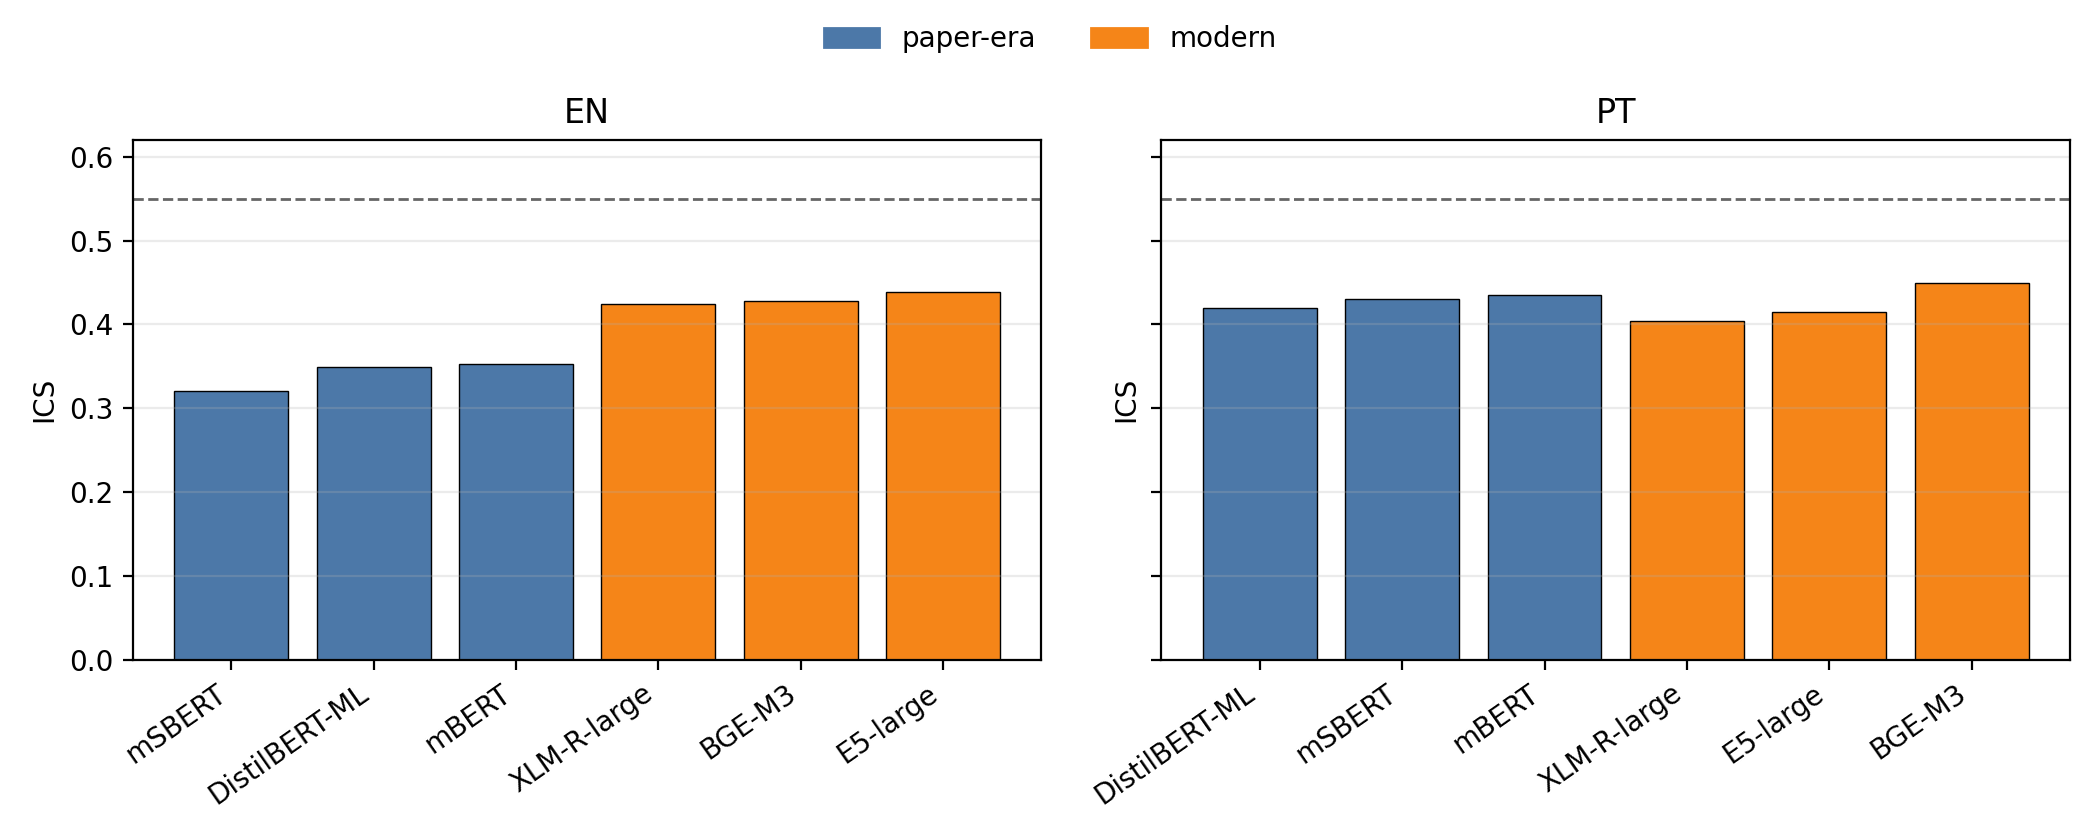
\includegraphics[width=\linewidth]{figures/ics_by_model_language.png}
\caption{Model-level ICS by language. No completed model crosses the 0.55 partial-capture
threshold. English shows a modest modern-model increase; Portuguese does not.}
\label{fig:ics}
\end{figure}

Table~\ref{tab:modeldiag} gives the model-level summary. The strongest English score is E5-large
(ICS 0.438), followed by BGE-M3 (0.428) and XLM-R-large (0.424). These are improvements over the
paper-era models, but still below the partial-capture threshold used in the repository analysis.
In Portuguese, the modern cohort does not improve the overall score: BGE-M3 is competitive, but
E5-large and XLM-R-large do not lift the language-level result.

\begin{table}[H]
\centering
\small
\begin{tabular}{llrrrr}
\toprule
Lang. & Model & ICS & LOD & AID & FLOOR \\
\midrule
EN & BGE-M3 & 0.428 & 0.069 & -0.041 & 0.430 \\
EN & E5-large & 0.438 & 0.091 & -0.018 & 0.803 \\
EN & XLM-R-large & 0.424 & 0.071 & -0.003 & 0.935 \\
EN & DistilBERT-ML & 0.349 & 0.181 & -0.044 & 0.744 \\
EN & mBERT & 0.353 & 0.205 & -0.045 & 0.777 \\
EN & mSBERT & 0.320 & 0.295 & -0.234 & 0.205 \\
PT & BGE-M3 & 0.449 & 0.055 & -0.035 & 0.417 \\
PT & E5-large & 0.415 & 0.201 & -0.035 & 0.826 \\
PT & XLM-R-large & 0.404 & 0.219 & -0.009 & 0.947 \\
PT & DistilBERT-ML & 0.419 & 0.191 & -0.040 & 0.779 \\
PT & mBERT & 0.435 & 0.191 & -0.037 & 0.795 \\
PT & mSBERT & 0.431 & 0.228 & -0.178 & 0.250 \\
\bottomrule
\end{tabular}
\caption{All completed model diagnostics averaged over naturalistic and neutral contexts. Positive
LOD means word-by-word literal alternatives still outperform the holistic synonym in idiomatic
cases; negative AID means the model does not prefer the holistic synonym over literal alternatives.}
\label{tab:modeldiag}
\end{table}

\begin{figure}[H]
\centering
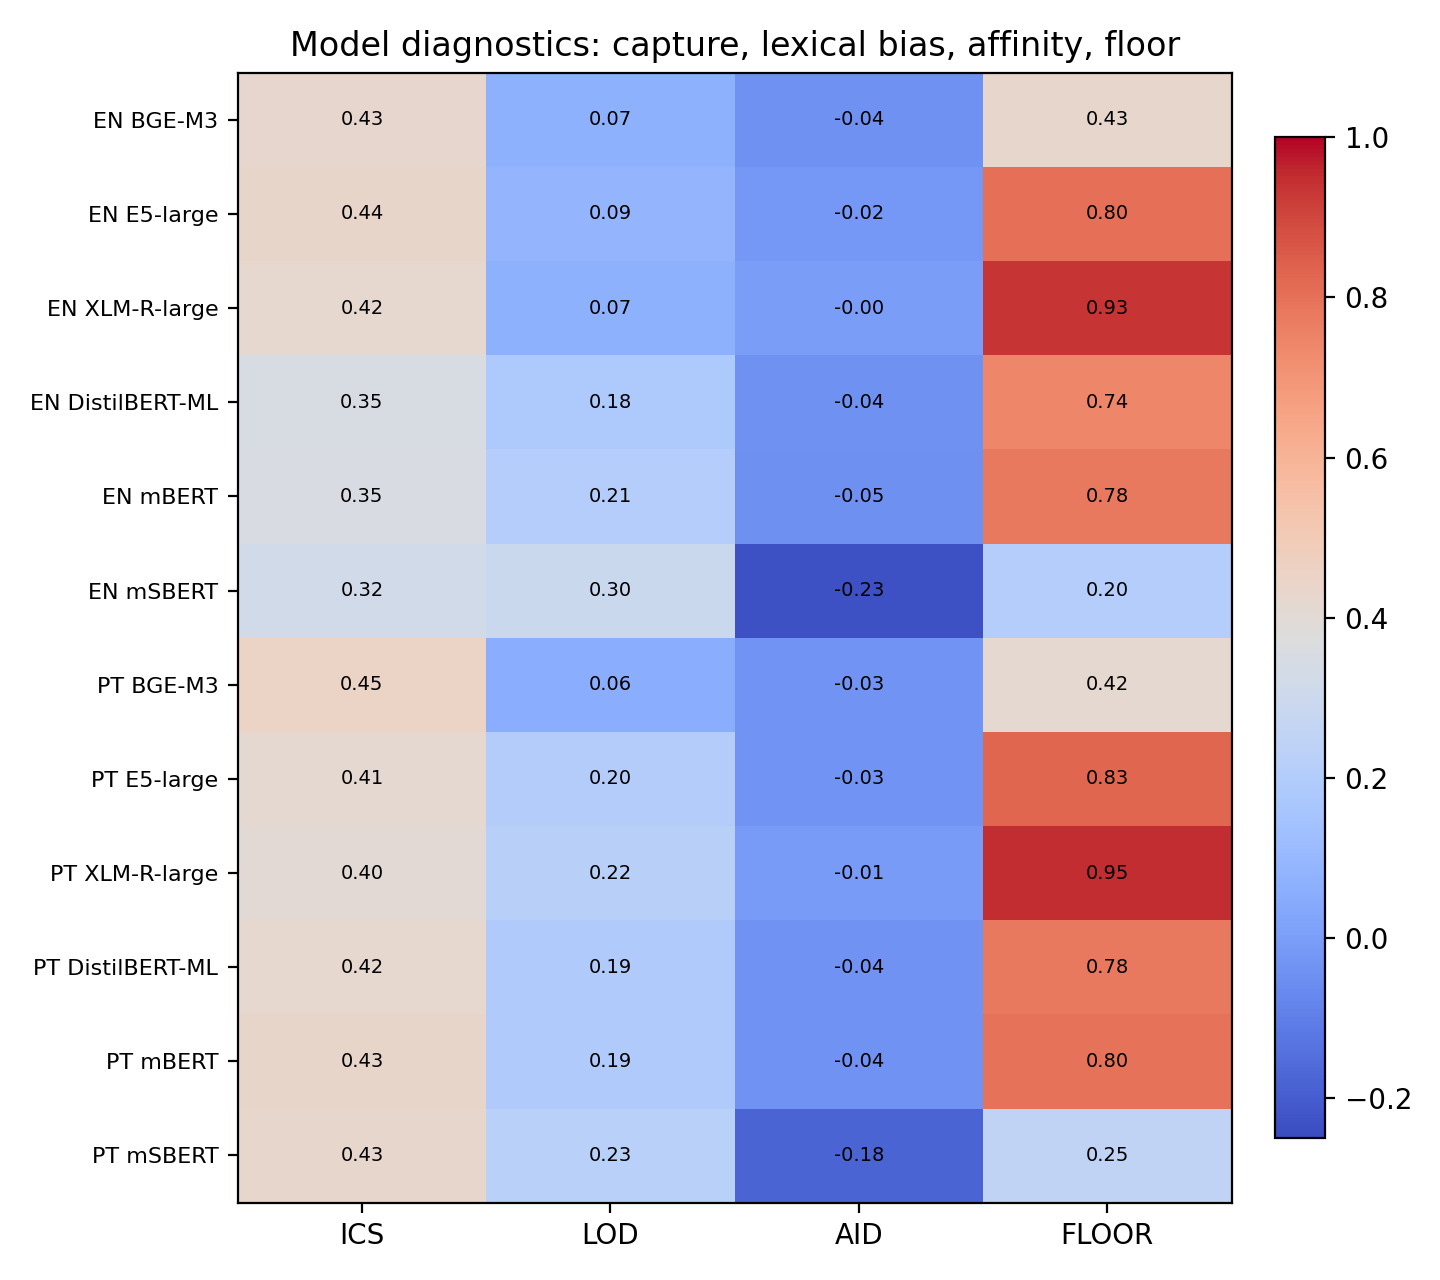
\includegraphics[width=0.82\linewidth]{figures/model_diagnostic_heatmap.png}
\caption{Diagnostic heatmap for the completed EN/PT cohort. XLM-R-large and E5-large have high
random-similarity floors in several conditions, while mSBERT has a lower floor but still shows
strong lexical component bias.}
\label{fig:diag}
\end{figure}

The core interpretation is therefore consistent with the original paper: newer models move the
English result in the right direction, but they do not solve idiomaticity representation. The
failure is not simply low capacity. Across models and languages, idiomatic NCs still tend to be
represented too close to literal component-based alternatives.

\section{Decoder-Only LLM Cohort}

We extend the study to a cohort of decoder-only LLMs spanning two generations and both base and
instruction-tuned variants: Qwen3 (2025) and Qwen3.5 (2026)~\cite{qwen3}, and Gemma~3 (2025) and
Gemma~4 (2026)~\cite{gemma3}, from 0.8B to 12B parameters. All are probed under the same NCIMP
English protocol at contextual-span (NC) level, averaging sub-token representations over the last
four layers (paper~\S3.2.1).

\paragraph{Extraction across runtimes.} Standard-attention models run through the HuggingFace/torch
path. Two practical obstacles required an Apple-MLX path: Qwen3.5 uses linear attention whose fast
kernels are CUDA-only (the torch fallback is unusably slow on macOS), and Gemma~4 is a unified
multimodal (\texttt{gemma4\_unified}) architecture. We therefore added an MLX embedder that loads
text LLMs via \texttt{mlx-lm} and multimodal ones via \texttt{mlx-vlm}, extracting the text
backbone's last four decoder-layer outputs by transparently recording them during the model's own
forward pass. Crucially, decoder-LLM layer outputs are the \emph{un-normalized} residual stream;
for Gemma in particular this residual is pathologically anisotropic (pairwise cosine of unrelated
texts $>0.98$) until the model's final RMSNorm is applied. We therefore apply the model's own final
norm to the last-four-layer average, which restores a comparable representation (Gemma's NC-level
random floor drops from $\approx0.98$ to $\approx0.6$). Base checkpoints are preferred where
available; instruction-tuned variants are labelled as such, since alignment tuning reshapes the
representation geometry.

Table~\ref{tab:llm} reports the cohort, sorted by capture score.

\begin{table}[H]
\centering
\small
\begin{tabular}{lllrrrr}
\toprule
Model & Gen. & Type & ISC & LOD & FLOOR & ICS \\
\midrule
Qwen3.5-0.8B-Base & 2026 & base/mlx & +0.186 & +0.101 & 0.561 & 0.425 \\
Qwen3.5-2B-it & 2026 & instruct/mlx & +0.200 & +0.060 & 0.511 & 0.444 \\
Gemma3-1B-it & 2025 & instruct/mlx & +0.207 & +0.080 & 0.667 & 0.455 \\
Qwen3.5-9B-it & 2026 & instruct/mlx & +0.217 & +0.010 & 0.540 & 0.478 \\
Qwen3-4B-Base & 2025 & base/torch & +0.188 & +0.050 & 0.825 & 0.479 \\
Qwen3.5-4B-it & 2026 & instruct/mlx & +0.222 & +0.011 & 0.523 & 0.479 \\
Gemma4-E2B-Base & 2026 & base/torch & +0.213 & +0.025 & 0.812 & 0.490 \\
Gemma3-12B-pt & 2025 & base/mlx & +0.258 & -0.006 & 0.556 & 0.498 \\
Gemma3-4B-pt & 2025 & base/mlx & +0.254 & +0.008 & 0.682 & 0.499 \\
Gemma4-12B-it & 2026 & instruct/mlx & -0.006 & +0.010 & 0.949 & 0.520 \\
Gemma4-12B-base & 2026 & base/mlx & +0.260 & -0.033 & 0.531 & 0.525 \\
\bottomrule
\end{tabular}
\caption{Decoder-only LLMs on English NCIMP at contextual-span (NC) level, averaged over
naturalistic and neutral contexts, using the last-four-layer + final-norm recipe. ISC is idiomatic
synonym capture, LOD lexical-overlap dominance, FLOOR the random-similarity floor (anisotropy
proxy), and ICS the composite capture score; the partial-capture threshold is 0.55. Numbers are
generated automatically from the run outputs.}
\label{tab:llm}
\end{table}

Three readings stand out. First, \emph{no model, in any generation, crosses the 0.55
partial-capture threshold}: the whole cohort clusters around ICS $0.42$--$0.53$, alongside the 2024
encoders. Second, \emph{the failure mode shifts}: decoder-only models drive lexical-overlap
dominance close to zero (unlike encoders, whose LOD stays clearly positive), so the residual
limitation is less ``idiom = sum of parts'' and more an anisotropic space with a small surviving
synonym--random separation. Third, \emph{the newest base model is the best and the only one to show
the right qualitative signs, yet it still stops short of the threshold}: the genuine cohort leader
(by ISC and by a healthy random floor) is base Gemma~4-12B at ICS $0.525$, which is also the only
model whose mean lexical-overlap dominance turns negative (LOD $=-0.03$) and whose mean idiomatic
affinity turns positive (AID $=+0.01$)---i.e.\ it actually prefers the holistic gold synonym over
the literal word-by-word one. In a like-for-like base comparison at 12B it modestly beats the 2025
Gemma~3-12B ($0.498$), so the newer generation does help a little; but the gain is small and the
score remains under partial capture. Meanwhile scaling within a generation saturates (Qwen3.5 stalls
from $\approx$4B onward at the 2025 Qwen3-4B value). The overall picture is a soft ceiling near
$0.50$--$0.53$ that more scale, a newer generation, and instruction tuning all approach but none
cross---strong evidence that the limitation is structural rather than a matter of capacity.

\paragraph{A metric caveat surfaced by extreme anisotropy.} The composite ICS divides by
$1-\text{FLOOR}$ (it is built on scaled similarity), so it becomes unstable as FLOOR$\to1$. The
instruction-tuned Gemma~4-12B is the clearest case: alignment tuning collapses its space (FLOOR
$\approx0.96$ even after the last-four-layer + norm recipe), its genuine synonym recovery (ISC) is
$\approx0$, yet the composite is buoyed to a misleadingly high value because the component
indicators go ``neutral.'' We therefore report FLOOR alongside ICS throughout and read any
high-FLOOR score with caution; the genuine cohort leader is a base model with a healthy floor, not
the collapsed instruct model.

\section{Preliminary Modern Embedding Models}

We also ran a cohort of recent (2025--2026) sentence-embedding models on the same English NCIMP
data. These models return a single pooled vector per input, so at NC level the diagnostics use an
\emph{isolated-phrase} embedding (the span text encoded on its own) rather than a contextual token
span; results should be read with that distinction in mind. Three runs have completed:
Qwen3-Embedding-0.6B, Qwen3-Embedding-4B, and multilingual-E5-large-instruct. Larger or newer
entries (Qwen3-Embedding-8B, Microsoft Harrier-OSS, NVIDIA llama-embed-nemotron-8B) are queued and
will be added with the same diagnostics; the asset builder picks up each run automatically.

\begin{table}[H]
\centering
\small
\begin{tabular}{lrrrrr}
\toprule
Model & ISC & LOD & AID & FLOOR & ICS \\
\midrule
Qwen3-Embedding-4B & 0.300 & 0.043 & -0.019 & 0.509 & 0.478 \\
mE5-large-instruct & 0.316 & 0.091 & -0.014 & 0.834 & 0.460 \\
Qwen3-Embedding-0.6B & 0.201 & 0.149 & -0.065 & 0.543 & 0.401 \\
\bottomrule
\end{tabular}
\caption{Completed modern sentence-embedding models on English NCIMP, isolated-phrase (NC) level,
averaged over naturalistic and neutral contexts. Qwen3-Embedding-4B matches the best decoder-only
score (ICS 0.478) and again shows the lowest lexical-overlap dominance (LOD 0.043), yet stays below
the 0.55 partial-capture threshold.}
\label{tab:emb}
\end{table}

Two patterns reinforce the earlier findings. First, the strongest modern models from very different
families converge: Qwen3-Embedding-4B (ICS 0.478) and the base decoder-only Qwen3-4B (ICS 0.479)
land at essentially the same capture score, both with near-zero lexical-overlap dominance and both
below threshold. Second, the random-similarity floor varies sharply by model: the Qwen3 embedding
models occupy a less anisotropic space (FLOOR $\approx$ 0.51--0.54) than mE5-large-instruct
(FLOOR 0.834), yet this lower anisotropy does not translate into crossing the capture threshold.
Taken together, neither reducing component bias nor reducing anisotropy is, on its own, sufficient
for idiomatic capture.

\section{Ordinary Perturbation Control}

The ordinary-control experiment asks whether the same synonym-random contrast works on
non-idiomatic targets. The expanded set contains 64 manually constructed examples: 16 idiomatic
NCs, 16 compositional NCs, 16 ordinary two-word phrases, and 16 ordinary single words. Examples
include \emph{doctor} $\rightarrow$ \emph{physician}/\emph{carpet},
\emph{apple} $\rightarrow$ \emph{fruit}/\emph{engine}, and
\emph{red car} $\rightarrow$ \emph{crimson vehicle}/\emph{coffee spoon}, plus varied targets from
domains such as occupations, nature, institutions, technology, transport, artifacts, and abstract
concepts.
Each substitution is evaluated at three levels: full sentence, contextual span after encoding the
full sentence, and isolated phrase.

\begin{figure}[H]
\centering
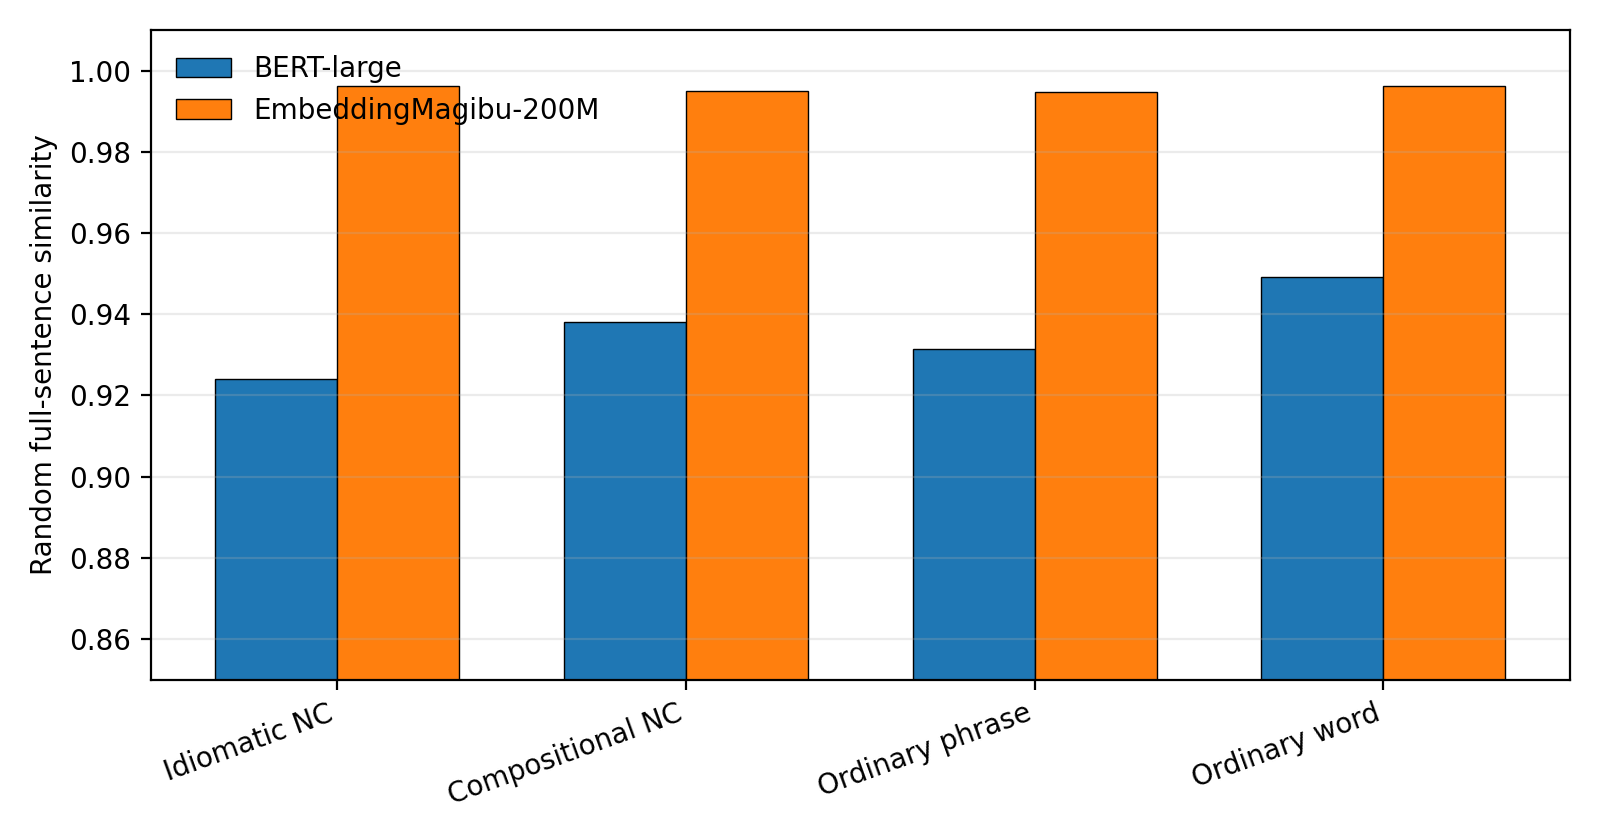
\includegraphics[width=0.82\linewidth]{figures/random_sentence_floor.png}
\caption{Random full-sentence similarities in the ordinary-control experiment. Random substitutions
remain highly similar across ordinary and NC groups, especially for the local embedding model. This
supports the concern that full-sentence similarity is not a clean idiomaticity signal.}
\label{fig:sentfloor}
\end{figure}

The full-sentence result supports the methodological critique. With BERT-large, random
full-sentence similarities are 0.924 for idiomatic NCs, 0.938 for compositional NCs, 0.931 for
ordinary two-word controls, and 0.949 for ordinary single-word controls. With
EmbeddingMagibu-200M, the same random similarities are even higher, around 0.995--0.996. This
shows that a shared sentence frame can dominate sentence-level cosine similarity.

The contextual-span result is more informative. Table~\ref{tab:ocg} reports raw contextual
synonym-random gaps and the proposed ordinary-calibrated gap. For BERT-large, the ordinary baseline
gap is 0.232. Idiomatic NCs reach only 0.088, or 0.378 of the ordinary baseline. Compositional NCs
reach 0.214, or 0.922 of the ordinary baseline. For the local embedding model, the contextual
ordinary baseline is smaller (0.072), and the idiomatic gap is negative, meaning that the random
replacement is on average closer than the holistic synonym.

\begin{table}[H]
\centering
\small
\begin{tabular}{llrrr}
\toprule
Model & Group & Syn. span & Rand. span & OCG \\
\midrule
BERT-large & Idiomatic NC & 0.753 & 0.665 & 0.378 \\
BERT-large & Compositional NC & 0.931 & 0.717 & 0.922 \\
BERT-large & Ordinary phrase & 0.893 & 0.687 & 0.886 \\
BERT-large & Ordinary word & 0.894 & 0.636 & 1.114 \\
EmbeddingMagibu-200M & Idiomatic NC & 0.948 & 0.949 & -0.025 \\
EmbeddingMagibu-200M & Compositional NC & 0.967 & 0.892 & 1.048 \\
EmbeddingMagibu-200M & Ordinary phrase & 0.957 & 0.905 & 0.723 \\
EmbeddingMagibu-200M & Ordinary word & 0.960 & 0.869 & 1.277 \\
\bottomrule
\end{tabular}
\caption{Contextual-span synonym and random similarities with ordinary-calibrated gap (OCG).
OCG is normalized by the equal-weight average synonym-random gap of ordinary single-word and
ordinary two-word controls for the same model and level.}
\label{tab:ocg}
\end{table}

\begin{figure}[H]
\centering
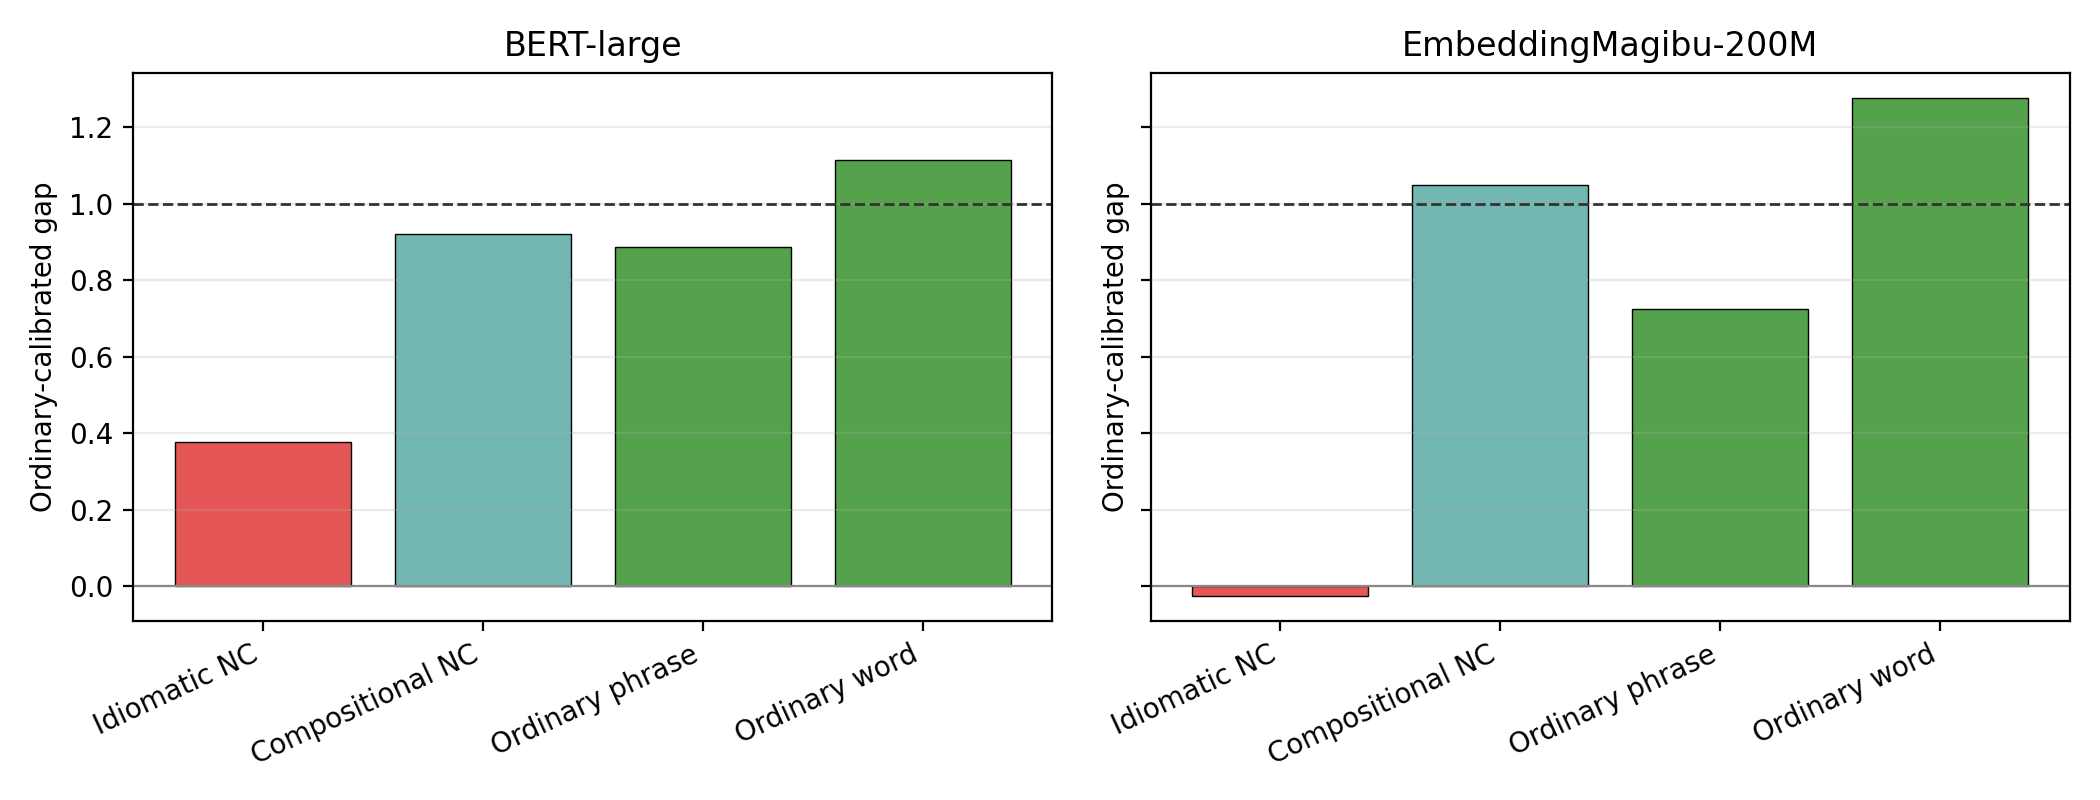
\includegraphics[width=\linewidth]{figures/ordinary_calibrated_contextual_gap.png}
\caption{Ordinary-calibrated contextual-span gaps. The dashed line marks ordinary-level separation.
BERT-large separates ordinary controls well but idiomatic NCs reach only about 38\% of that
baseline. The local embedding model shows an even stronger failure for idiomatic NCs.}
\label{fig:ocg}
\end{figure}

This is the central new point. The problem is not that all local substitutions are equally
invisible. BERT-large can distinguish ordinary synonyms from random replacements at the contextual
span level. The separation is specifically much weaker for idiomatic NCs. Therefore, the ordinary
control strengthens the idiomaticity interpretation at span level while weakening any argument that
relies on raw full-sentence similarity.

\paragraph{The control across all twenty models.} We ran the ordinary-control protocol for the full
study cohort---the six encoders/embeddings, the three modern embedding models, and the eleven
decoder LLMs---and summarise each model by its ordinary-calibrated gap
$\mathrm{OCG}_{\mathrm{idiom}}=\Delta_{\mathrm{idiom}}/\Delta_{\mathrm{Ord}}$ at the contextual-span
level (Figure~\ref{fig:ocg-all}). The result is uniform: \emph{no model reaches}
$\mathrm{OCG}_{\mathrm{idiom}}=1$ (the best, base Gemma~4-12B, is $0.68$), whereas the
\emph{compositional} calibrated gap sits at or above $1$ for nearly every model. The paper-era
encoders are worst, at $\mathrm{OCG}_{\mathrm{idiom}}\approx 0$ or slightly negative (mBERT $-0.10$,
XLM-R $-0.01$): for them an idiomatic gold synonym is no closer to the target than a random
replacement, even though the same models separate ordinary \emph{doctor}$\rightarrow$\emph{physician}
from \emph{doctor}$\rightarrow$\emph{carpet} cleanly. This is the strongest single piece of evidence
that the failure is specific to idiomaticity rather than a generic insensitivity of the
embedding--cosine setup.

\begin{figure}[H]
\centering
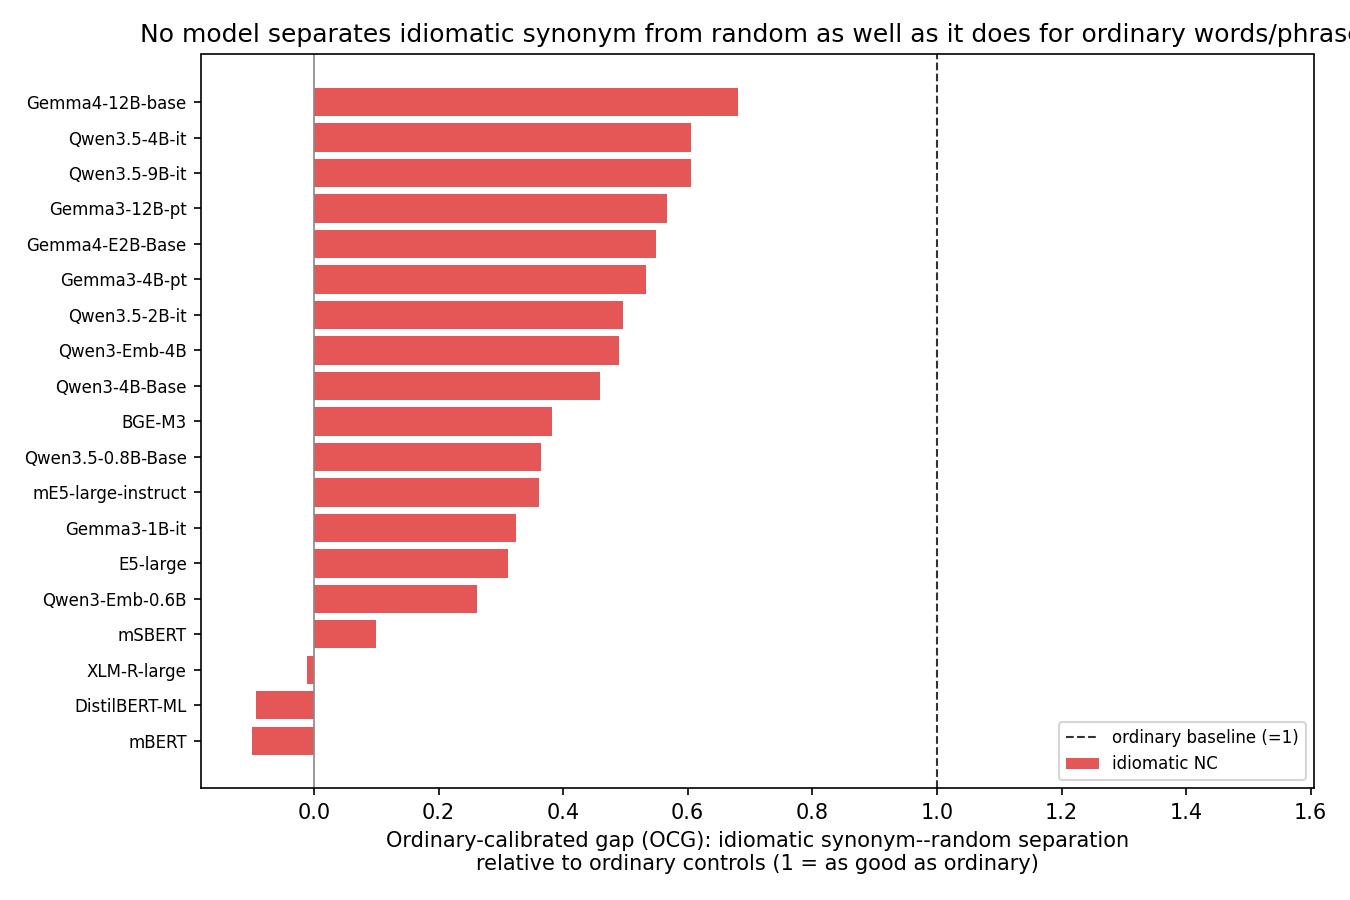
\includegraphics[width=0.92\linewidth]{figures/ocg_all_models.png}
\caption{Ordinary-calibrated idiomatic gap (OCG) for all 20 models at contextual-span level. The
dashed line at 1 marks the ordinary-control baseline (idiomatic separation as good as ordinary
words/phrases). Every model falls short; the newest base LLM (Gemma~4-12B) is closest at 0.68, the
2024 encoders are near or below zero. Gemma~4-12B-it is omitted (its collapsed space makes the ratio
unstable).}
\label{fig:ocg-all}
\end{figure}

\section{What Was Included and What Was Not}

All result files currently present in the worktree were inspected. The main scientific claims use
the completed EN/PT six-model NCIMP runs and the two ordinary-perturbation runs. The mBERT pilot is
reported as a reproduction sanity check and is also contained in the English full cohort. The smoke
and deterministic mock outputs are validation artifacts, not model-evidence about idiomaticity.

The model registry also contains entries for newer embedding or LLM-style models, including Qwen3
Embedding variants, multilingual E5-instruct, GTE-Qwen2, NV-Embed-v2, llama-embed-nemotron, BGE
ICL, Qwen3 base LLMs, and Gemma 4 text-path adapters. Of these, one decoder-only run and three
modern sentence-embedding runs are complete and reported here as preliminary results
(Qwen3-4B-Base, Table~\ref{tab:llm}; Qwen3-Embedding-0.6B/4B and mE5-large-instruct,
Table~\ref{tab:emb}), all on English. The remaining entries (Qwen3.5 and Gemma~4 text paths,
Qwen3-Embedding-8B, Harrier-OSS, llama-embed-nemotron) are still downloading or running at the time
of writing and are not claimed as results unless a corresponding result CSV is present. They will be reported as a full decoder-only and
modern-embedding cohort once their runs finish and the same diagnostics are generated; the asset
builder already picks up each decoder-only run automatically as its \texttt{indicators.csv} appears.

\section{Discussion}

The combined evidence supports a careful middle position. The original idiomaticity probe is not
invalidated by the ordinary-control pilot. Rather, the pilot clarifies where the evidence is strong.
At full-sentence level, the measurement is too insensitive to local perturbations: random
substitutions remain highly similar even for ordinary words and phrases. At contextual-span level,
BERT-large preserves a robust synonym-random distinction for ordinary controls, but that distinction
collapses for idiomatic NCs. This pattern is exactly what an idiomaticity-specific failure should
look like.

The modern-model replication adds a second conclusion. Newer models show a modest English gain, but
not a robust multilingual gain. The persistent positive LOD and negative AID indicate structural
lexical-compositional bias: models still overweight the literal components of an idiom when the
target should be represented holistically. The ordinary-calibrated metric makes this easier to
explain because it avoids asking whether a raw cosine value is ``high'' or ``low'' in isolation. It
asks instead: compared with ordinary substitutions, how much synonym-random separation is left for
idiomatic expressions?

The preliminary decoder-only result refines this picture. Among all completed models, the base
Qwen3-4B-Base most reduces the lexical-component bias (lowest LOD, affinity nearest zero) and reaches
the highest capture score, yet it still does not cross the partial-capture threshold. This suggests
that the encoder-era diagnosis---idioms represented as the sum of their parts---is not the whole
story for newer decoder-only models. Their remaining limitation looks more geometric: a highly
anisotropic space inflates all similarities, so even when component bias recedes, the surviving
synonym--random separation for idiomatic targets stays small. This is precisely the contrast the
ordinary-calibrated gap is designed to expose, and it motivates running the calibrated controls for
the decoder-only and modern-embedding cohorts as they complete.

\section{Limitations}

The ordinary-control experiment is still a pilot. It now uses 64 manually constructed examples,
but some random replacements are grammatically awkward after substitution. A larger version should
balance grammaticality, frequency, concreteness, length, syntactic fit, and semantic relatedness.
The proposed OCG metric also requires ordinary controls for every model and representation level;
the completed EN/PT NCIMP cohort cannot be retroactively ordinary-calibrated without running those
controls for the same models. Finally, sentence-embedding models and contextual-token models must
be kept separate. For sentence-embedding models, an NC-level run in this repository corresponds to
encoding the isolated phrase, not extracting a contextual token span from the full sentence.

\section{Conclusion}

Idiomaticity probing with minimal substitutions remains valuable, but it should be calibrated
against ordinary perturbation behavior. The current repository evidence supports three conclusions.
First, raw full-sentence similarity is too insensitive to local replacements to carry the argument
alone. Second, contextual-span similarity provides a stronger idiomaticity signal: ordinary controls
separate synonyms from random replacements much better than idiomatic NCs do. Third, modern
embedding and encoder models have not solved idiomaticity representation; progress is modest,
language-dependent, and still constrained by lexical component bias. A preliminary base
decoder-only model (Qwen3-4B-Base) most reduces that component bias and reaches the highest capture
score yet, but still falls short of partial capture, pointing to an anisotropy-and-residual-gap
limitation rather than a solved problem. The proposed ordinary-calibrated gap gives a direct way to
report this contrast as the decoder-only and modern-embedding cohorts complete.

\begin{thebibliography}{9}

\bibitem{he2025idiomaticity}
Wei He, Tiago Kramer Vieira, Marcos Garcia, Carolina Scarton, Marco Idiart, and Aline
Villavicencio.
\newblock Investigating idiomaticity in word representations.
\newblock \emph{Computational Linguistics}, 51(2):505--555, 2025.
\newblock doi:10.1162/coli\_a\_00546.

\bibitem{devlin2019bert}
Jacob Devlin, Ming-Wei Chang, Kenton Lee, and Kristina Toutanova.
\newblock BERT: Pre-training of deep bidirectional transformers for language understanding.
\newblock In \emph{Proceedings of NAACL-HLT}, pages 4171--4186, 2019.

\bibitem{conneau2020xlmr}
Alexis Conneau, Kartikay Khandelwal, Naman Goyal, Vishrav Chaudhary, Guillaume Wenzek,
Francisco Guzman, Edouard Grave, Myle Ott, Luke Zettlemoyer, and Veselin Stoyanov.
\newblock Unsupervised cross-lingual representation learning at scale.
\newblock In \emph{Proceedings of ACL}, pages 8440--8451, 2020.

\bibitem{reimers2019sbert}
Nils Reimers and Iryna Gurevych.
\newblock Sentence-BERT: Sentence embeddings using Siamese BERT-networks.
\newblock In \emph{Proceedings of EMNLP-IJCNLP}, pages 3982--3992, 2019.

\bibitem{qwen3}
Qwen Team, Alibaba Group.
\newblock Qwen3 technical report.
\newblock arXiv preprint, 2025.

\bibitem{gemma3}
Gemma Team, Google DeepMind.
\newblock Gemma 3 technical report.
\newblock arXiv preprint, 2025.

\end{thebibliography}

\end{document}
